%%%%%%%%%%%%%%%%%%%%%%%%%%%%%%%%%%%%%%%%%%%%%%%%%%%%%%%%%%%%
%%% ELIFE ARTICLE TEMPLATE
%%%%%%%%%%%%%%%%%%%%%%%%%%%%%%%%%%%%%%%%%%%%%%%%%%%%%%%%%%%%
%%% PREAMBLE 
\documentclass[9pt,lineno]{elife}
% Use the onehalfspacing option for 1.5 line spacing
% Use the doublespacing option for 2.0 line spacing
% Please note that these options may affect formatting.

\usepackage{lipsum} % Required to insert dummy text
\usepackage[version=4]{mhchem}
\usepackage{siunitx}
\DeclareSIUnit\Molar{M}

%%%%%%%%%%%%%%%%%%%%%%%%%%%%%%%%%%%%%%%%%%%%%%%%%%%%%%%%%%%%
%%% ARTICLE SETUP
%%%%%%%%%%%%%%%%%%%%%%%%%%%%%%%%%%%%%%%%%%%%%%%%%%%%%%%%%%%%
\title{Mapping sites of shifting and constant mutational effects on the evolutionary landscape of HIV Envelope}

\author[1,2\authfn{1}]{Hugh K. Haddox}
\author[1,2\authfn{1}]{Adam S. Dingens}
\author[1,3]{Sarah K. Hilton}
\author[4]{Julie Overbaugh}
\author[1,2,3]{Jesse D. Bloom}
\affil[1]{Basic Sciences Division and Computational Biology Program, Fred Hutchinson Cancer Research Center, Seattle, WA}
\affil[2]{Molecular and Cellular Biology PhD program, University of Washington, Seattle, WA}
\affil[3]{Department of Genome Sciences, University of Washington, Seattle, WA}
\affil[4]{Human Biology Division, Fred Hutchinson Cancer Research Center, Seattle, WA}
\contrib[\authfn{1}]{These authors contributed equally to this work}

\corr{jbloom@fredhutch.org}{JDB}
% \presentadd[\authfn{5}]{eLife Sciences editorial Office, eLife Sciences, Cambridge, United Kingdom}

%%%%%%%%%%%%%%%%%%%%%%%%%%%%%%%%%%%%%%%%%%%%%%%%%%%%%%%%%%%%
%%% ARTICLE START
%%%%%%%%%%%%%%%%%%%%%%%%%%%%%%%%%%%%%%%%%%%%%%%%%%%%%%%%%%%%

\begin{document}

\maketitle

\begin{abstract}
HIV Envelope (Env) evolves rapidly.
The immediate the evolutionary space accessible to any viral variant is largely determined by the effects of single amino-acid mutations.
However, the effects of these mutations can shift over evolutionary time as the virus traverses through sequence space.
Here we comprehensively quantify the ways in which mutational effects shift or remain constant by experimentally measuring the effects of all amino-acid mutations to two homologs of Env with 85\% (?) sequence identity.
We find...
\end{abstract}


\section{Introduction}


\section{Results}

\subsection*{Deep mutational scanning of two Env homologs from transmitted-founder (?) viruses}
Previously we've done deep mutational scanning on a lab-passaged CXCR4-tropic virus isolated late in infection.
Here we sought to examine the effects of mutations in viruses more relevant to selection on HIV in nature.
We chose...

The relationship between BG505 and BF520 is shown in \ref{ref:tree}

\begin{figure}
\centerline{\bf \Large A \hspace{0.52\textwidth} \bf B \hspace{0.35\textwidth}}
\centerline{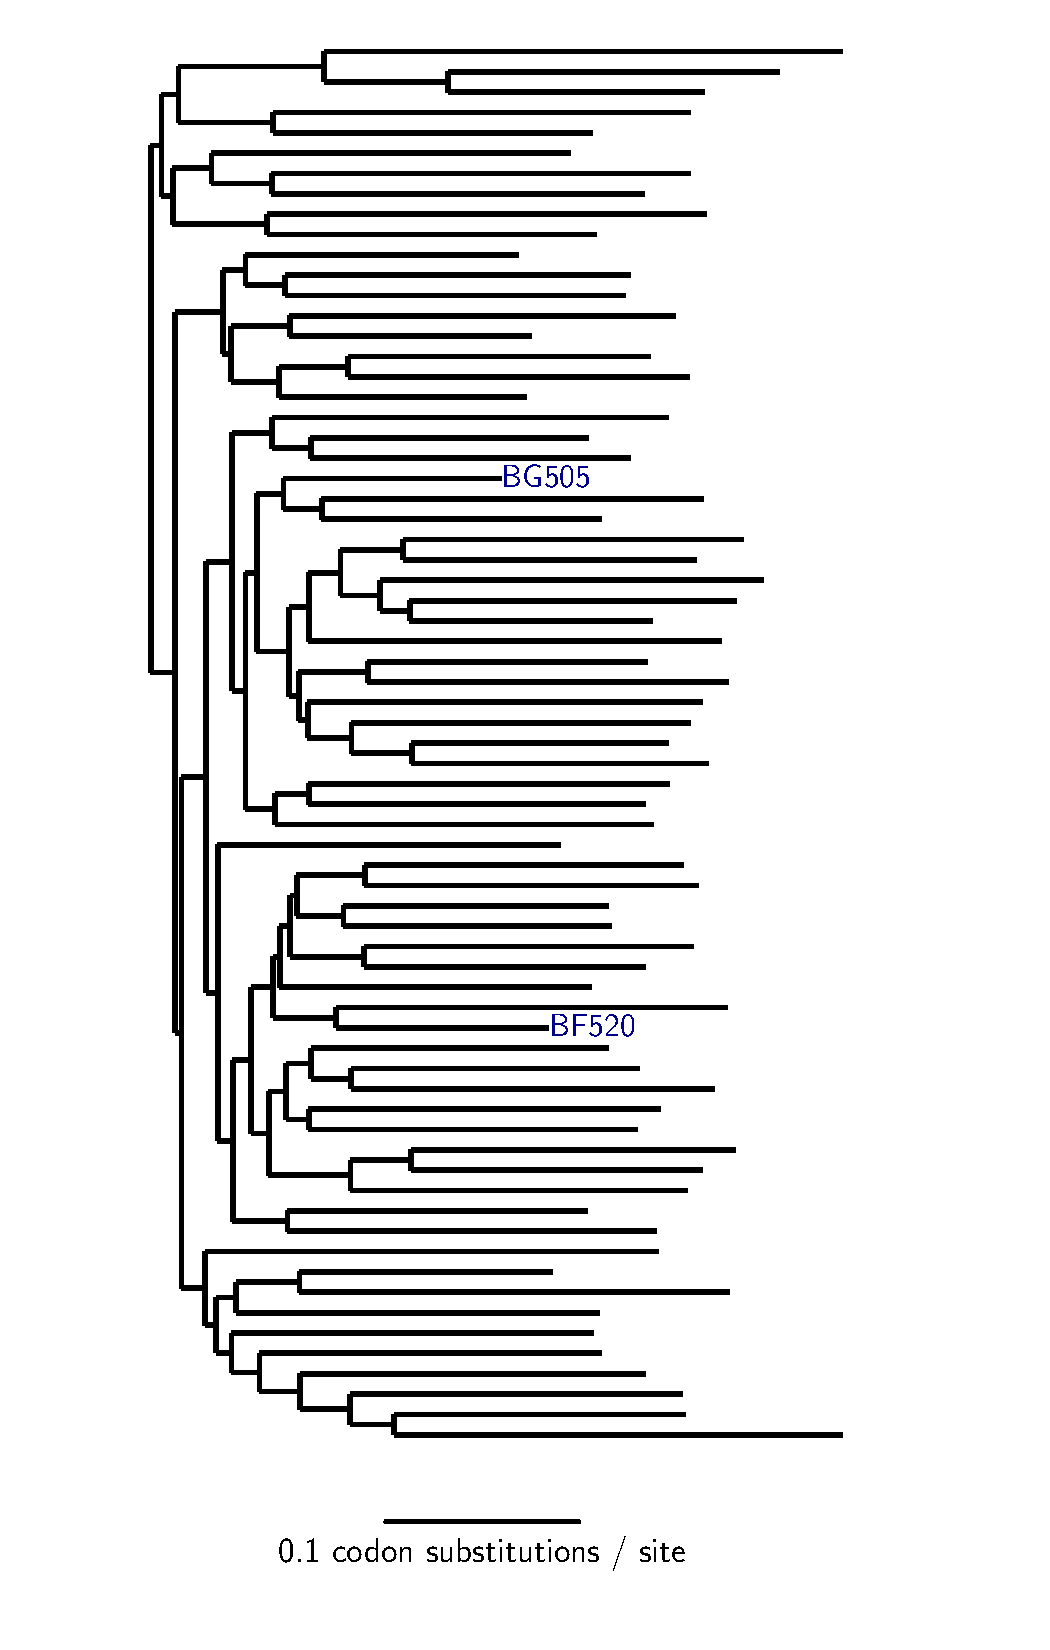
\includegraphics[width=0.6\textwidth]{figures/tree_plot.pdf} 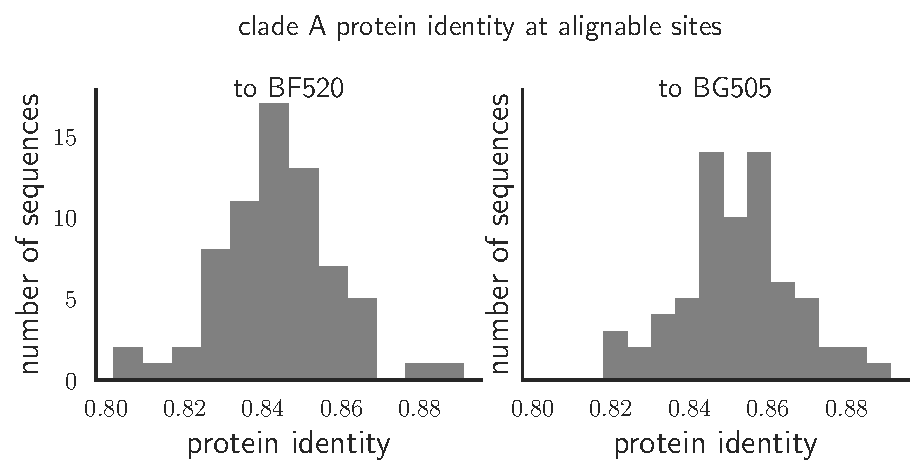
\includegraphics[width=0.4\textwidth]{figures/masked_alignment_identity.pdf}}
\caption{\label{fig:tree}
CAPTION
}
\figdata{The coding sequence alignment of clade A \textit{env} sequences in FASTA format is in \texttt{cladeA\_alignment.fasta}.}
\figdata{Sites masked in all phylogenetic analyses because they were not mutagenized in our experiments or are poorly alignable are listed in \texttt{alignment\_mask.csv}.}
\end{figure}

We performed deep mutational scanning as described previously with a few modifications that are very briefly described here and detailed in the methods.
We saw strong selection as indicated in \ref{fig:mutfreqs}.
More details on DMS is shown in \ref{suppfig:dms}

\begin{figure}
\centerline{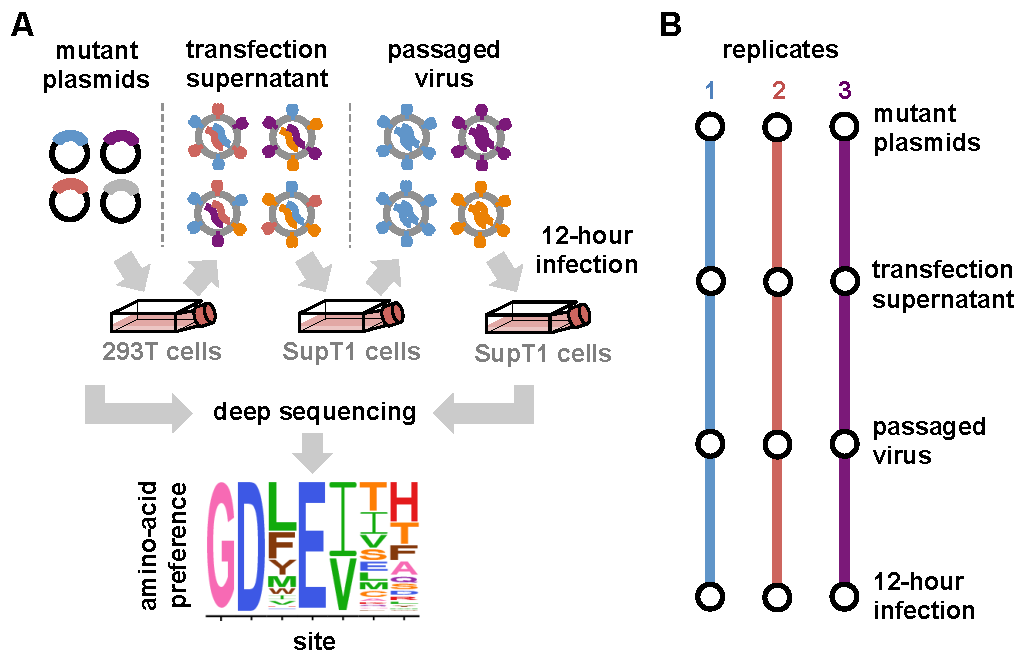
\includegraphics[width=0.9\textwidth]{figures/dms_schematic/dms_schematic.pdf}}
\caption{\label{fig:dms_schematic}
Deep mutational scanning workflow.
{\bf (A)} For each homolog, we made a library of proviral HIV plasmids with random codon-level mutations in \textit{env}.
We then transfected the plasmids into 293T cells to generate mutant viruses, which may lack a genotype-phenotype link since transfected cell are expected to each receive multiple plasmids.
To establish this link and select for functional variants, we first passaged the libraries in SupT1 cells at a low MOI.
Then, we imposed a second round of selection by infecting the passaged viruses into SupT1 cells at a high MOI and then harvesting reverse-transcribed unintegrated viral DNA at 12 hours post-infection.
Finally, we deep sequenced the libraries before and after selection.
We also deep sequenced wildtype controls to estimate error rates due to PCR, deep sequencing, and viral replication.
Using these sequencing data, we then inferred each site's preference for each of the 20 amino acids.
{\bf (B)} For each homolog, we conducted this experiment in full biological triplicate, beginning at the stage of independently creating the plasmid mutant libraries.
}
\end{figure}

\begin{figure}
{{\bf \Large A} \hspace{0.2\textwidth} BG505 \hspace{0.51\textwidth} BF520} \\
{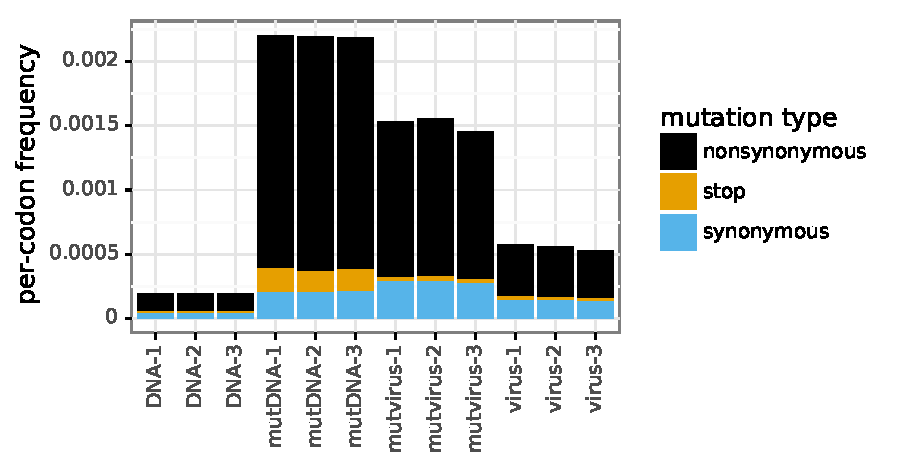
\includegraphics[height=0.32\textwidth]{figures/BG505_avgmutfreqs.pdf}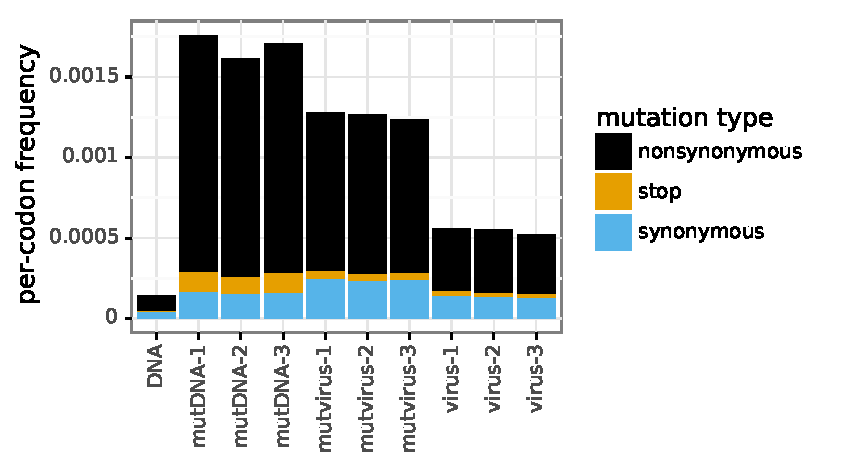
\includegraphics[clip=true,trim=0in 0in 1.7in 0in,height=0.32\textwidth]{figures/BF520_avgmutfreqs.pdf}} \\
{\bf \Large B} \\
{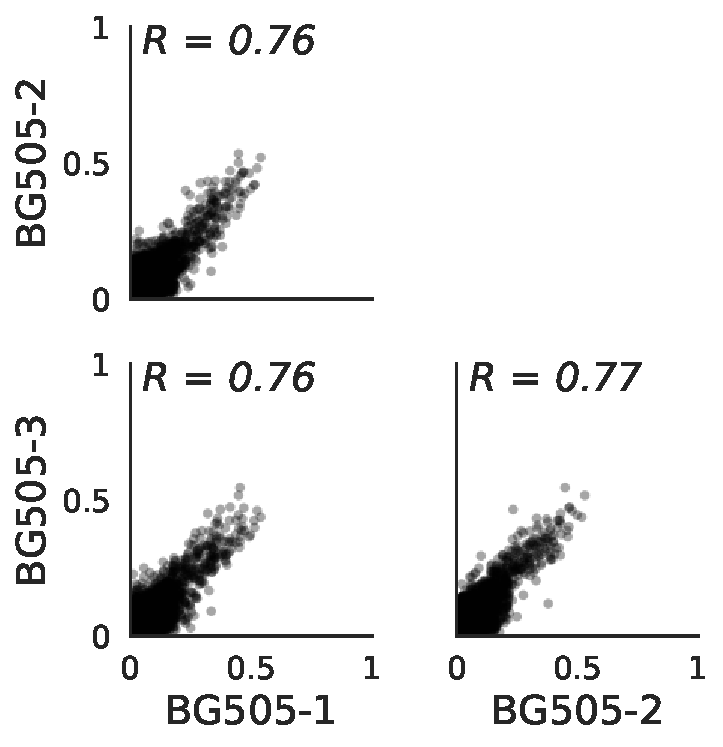
\includegraphics[width=0.37\textwidth]{figures/BG505_prefscorr.pdf}\hspace{0.1\textwidth}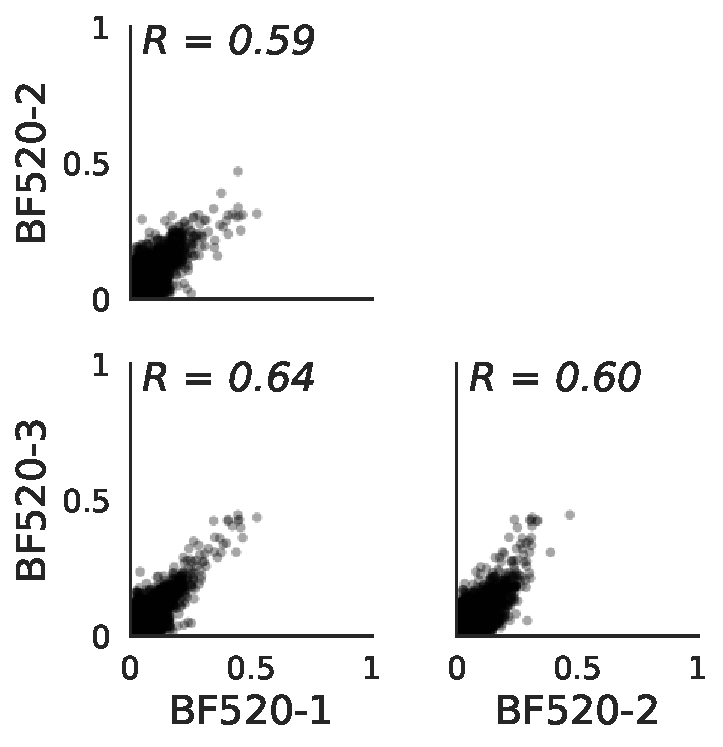
\includegraphics[width=0.37\textwidth]{figures/BF520_prefscorr.pdf}}
\caption{\label{fig:mutfreqs}
The deep mutational scanning experiments imposed strong purifying selection and led to reproducible estimates of each homolog's amino-acid preferences.
{\bf(A)} For each replicate of each homolog, we deep sequenced the starting plasmid libraries (DNA) and the selected virus libraries (virus).
Bars show the per-codon mutation frequency averaged across all sites after subtracting mutation frequencies determined using wildtype controls (Fig \ref{suppfig:ch3_mutfreqs_supp}).
Mutations leading to stop codons were purged during the selection step to 3-17\% their starting frequencies (see red numbers), indicating strong purifying selection.
Nonsynonymous mutations decreased to 40-50\% their starting frequencies, consistent with a large fraction of amino-acid mutations being deleterious to Env.
Synonymous mutations only decreased to 87-95\% their starting frequencies, as would be expected if synonymous mutations tend to have more neutral effects than nonsynonymous changes.
Panels {\bf(B)} and {\bf(C)} show the correlation in our estimates of each homolog's site-specific amino-acid preferences between experimental replicates, with {\bf(B)} showing the correlation between BF520 replicates and {\bf(C)} showing the correlation between BG505 replicates.
Each correlation plot reports the associated Pearson correlation coefficient, which ranged from 0.59-0.75, indicating that our estimates are largely repeatable between replicates.
}
\figdata{The raw numerical data plotted in panel (A) are in the file \texttt{avgmutfreqs.csv}.}
\figdata{The amino-acid preferences for each replicate and the replicate averages for each homolog are in \texttt{all\_prefs\_unscaled.zip}.}
\end{figure}


\subsection*{Re-scaling the experimental measurements to optimally describe HIV evolution in nature}

Re-scaled as in \ref{tab:phydms}

\begin{table}
\begin{fullwidth}
{\centering \begin{tabular}{lrrrrrrrrr}
\toprule
           Model &  $\Delta$AIC &  LogLikelihood &  nParams &  stringency &  $\overline{\omega}$ &  $\omega_{\alpha}$ &  $\omega_{\beta}$ &  nsites $\omega_r > 1$ &  nsites $\omega_r < 1$ \\
\midrule
     ExpCM BF520 &          0.0 &       -35218.8 &        7 &         2.8 &                  1.4 &                1.0 &               0.7 &                     66 &                     35 \\
     ExpCM BG505 &        269.0 &       -35353.3 &        7 &         2.1 &                  1.3 &                0.9 &               0.7 &                     65 &                     53 \\
 Goldman-Yang M5 &       3455.1 &       -36941.4 &       12 &         nan &                  0.8 &                0.6 &               0.7 &                     14 &                    211 \\
\bottomrule
\end{tabular}
}
\caption{\label{tab:phydms}
Phylogenetic models that incorporate Env's preferences indicate that selection was less stringent in the lab than in nature.}
\tabledata{Results for phylogenetic models where $\omega$ is not drawn from a gamma-distribution or where the preferences are averaged across sites are in \texttt{modelcomparison.md}.}
\end{fullwidth}
\end{table}

\begin{figure}
\centerline{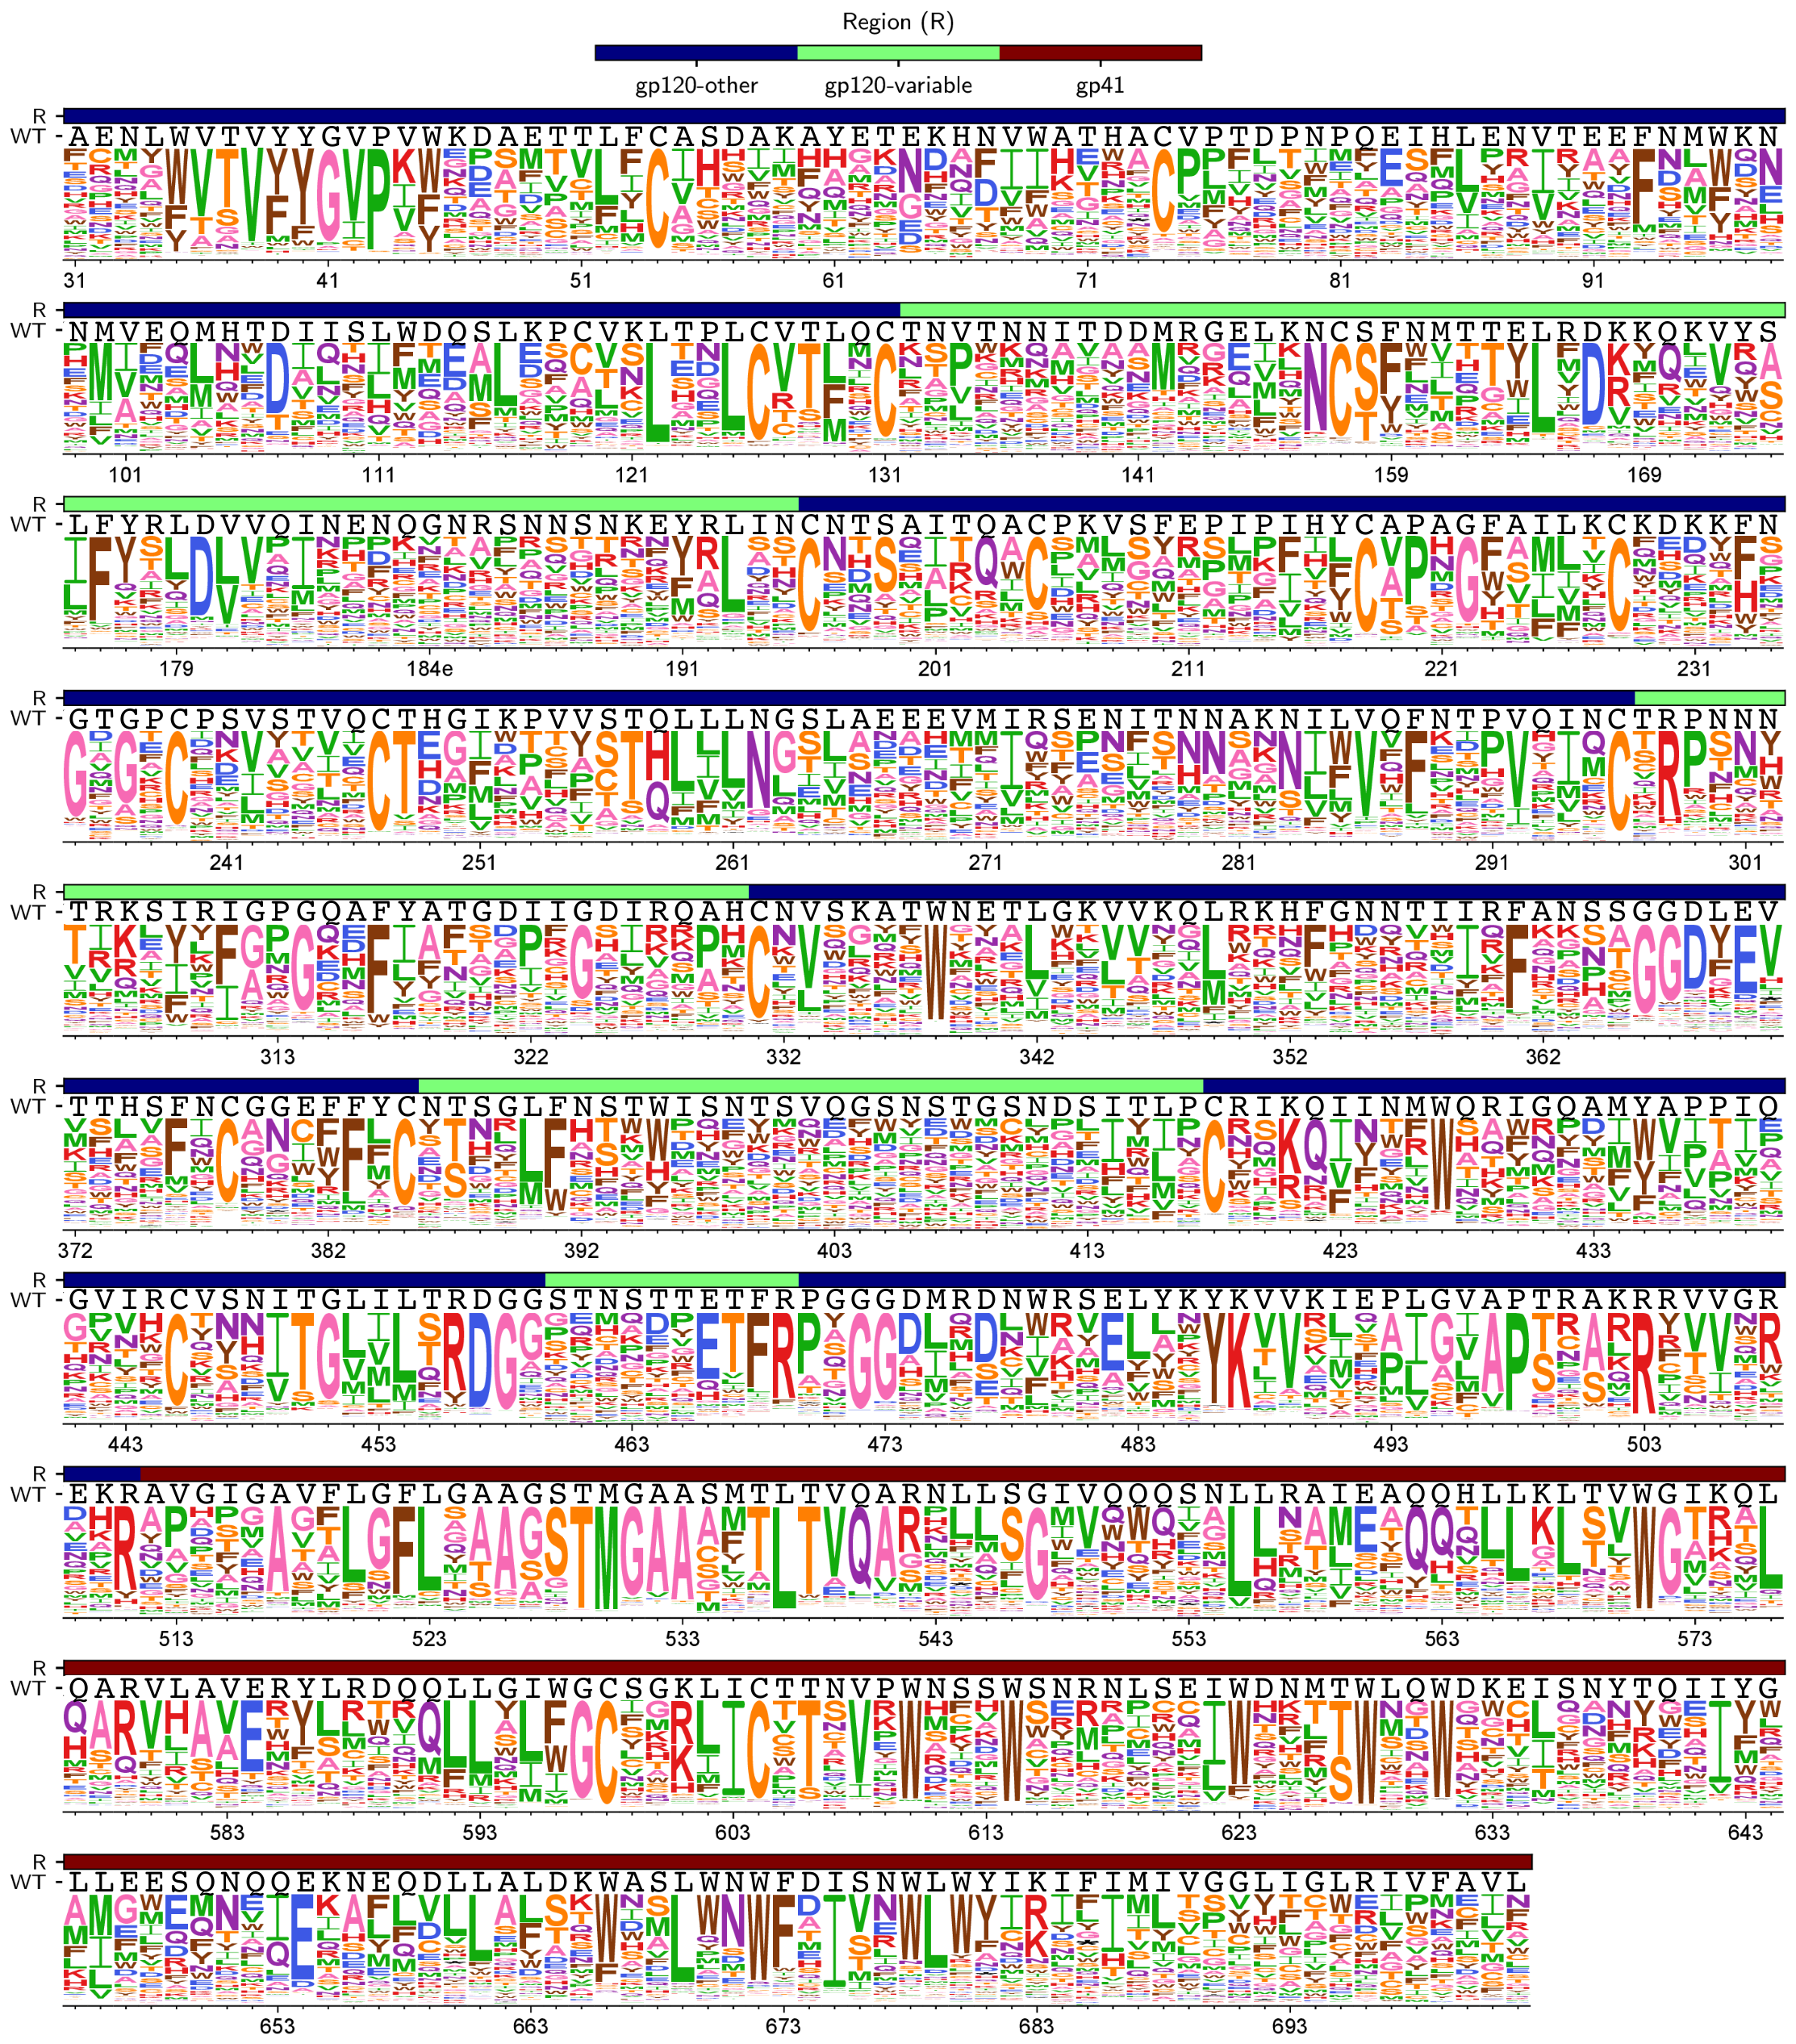
\includegraphics[width=6.5in]{figures/prefs_BG505/prefs_BG505.png}}
\caption{\label{fig:bg505_prefs_logo}
The rescaled averaged site-specific amino-acid preferences for BG505.
This logo plot shows the site-specific amino-acid preferences for BG505 after averaging between replicates and then rescaling them using the stringency parameter from Table \ref{tab:phydms} inferred for BG505 from the group-M alignment.
Each site has a stack of 20 letters corresponding to the 20 amino acids.
Letter heights, which sum to one at each site, are proportional to the site's preference for each amino acid.
The top bar (R) indicates gp120 variable loops, other regions in gp120, or gp41.
The bottom bar (WT) shows the wildtype amino-acid sequence for BG505.
Sites are numbered according to the HXB2 numbering scheme~\cite{korber1998numbering}).
}
\end{figure}

\begin{figure}
\centerline{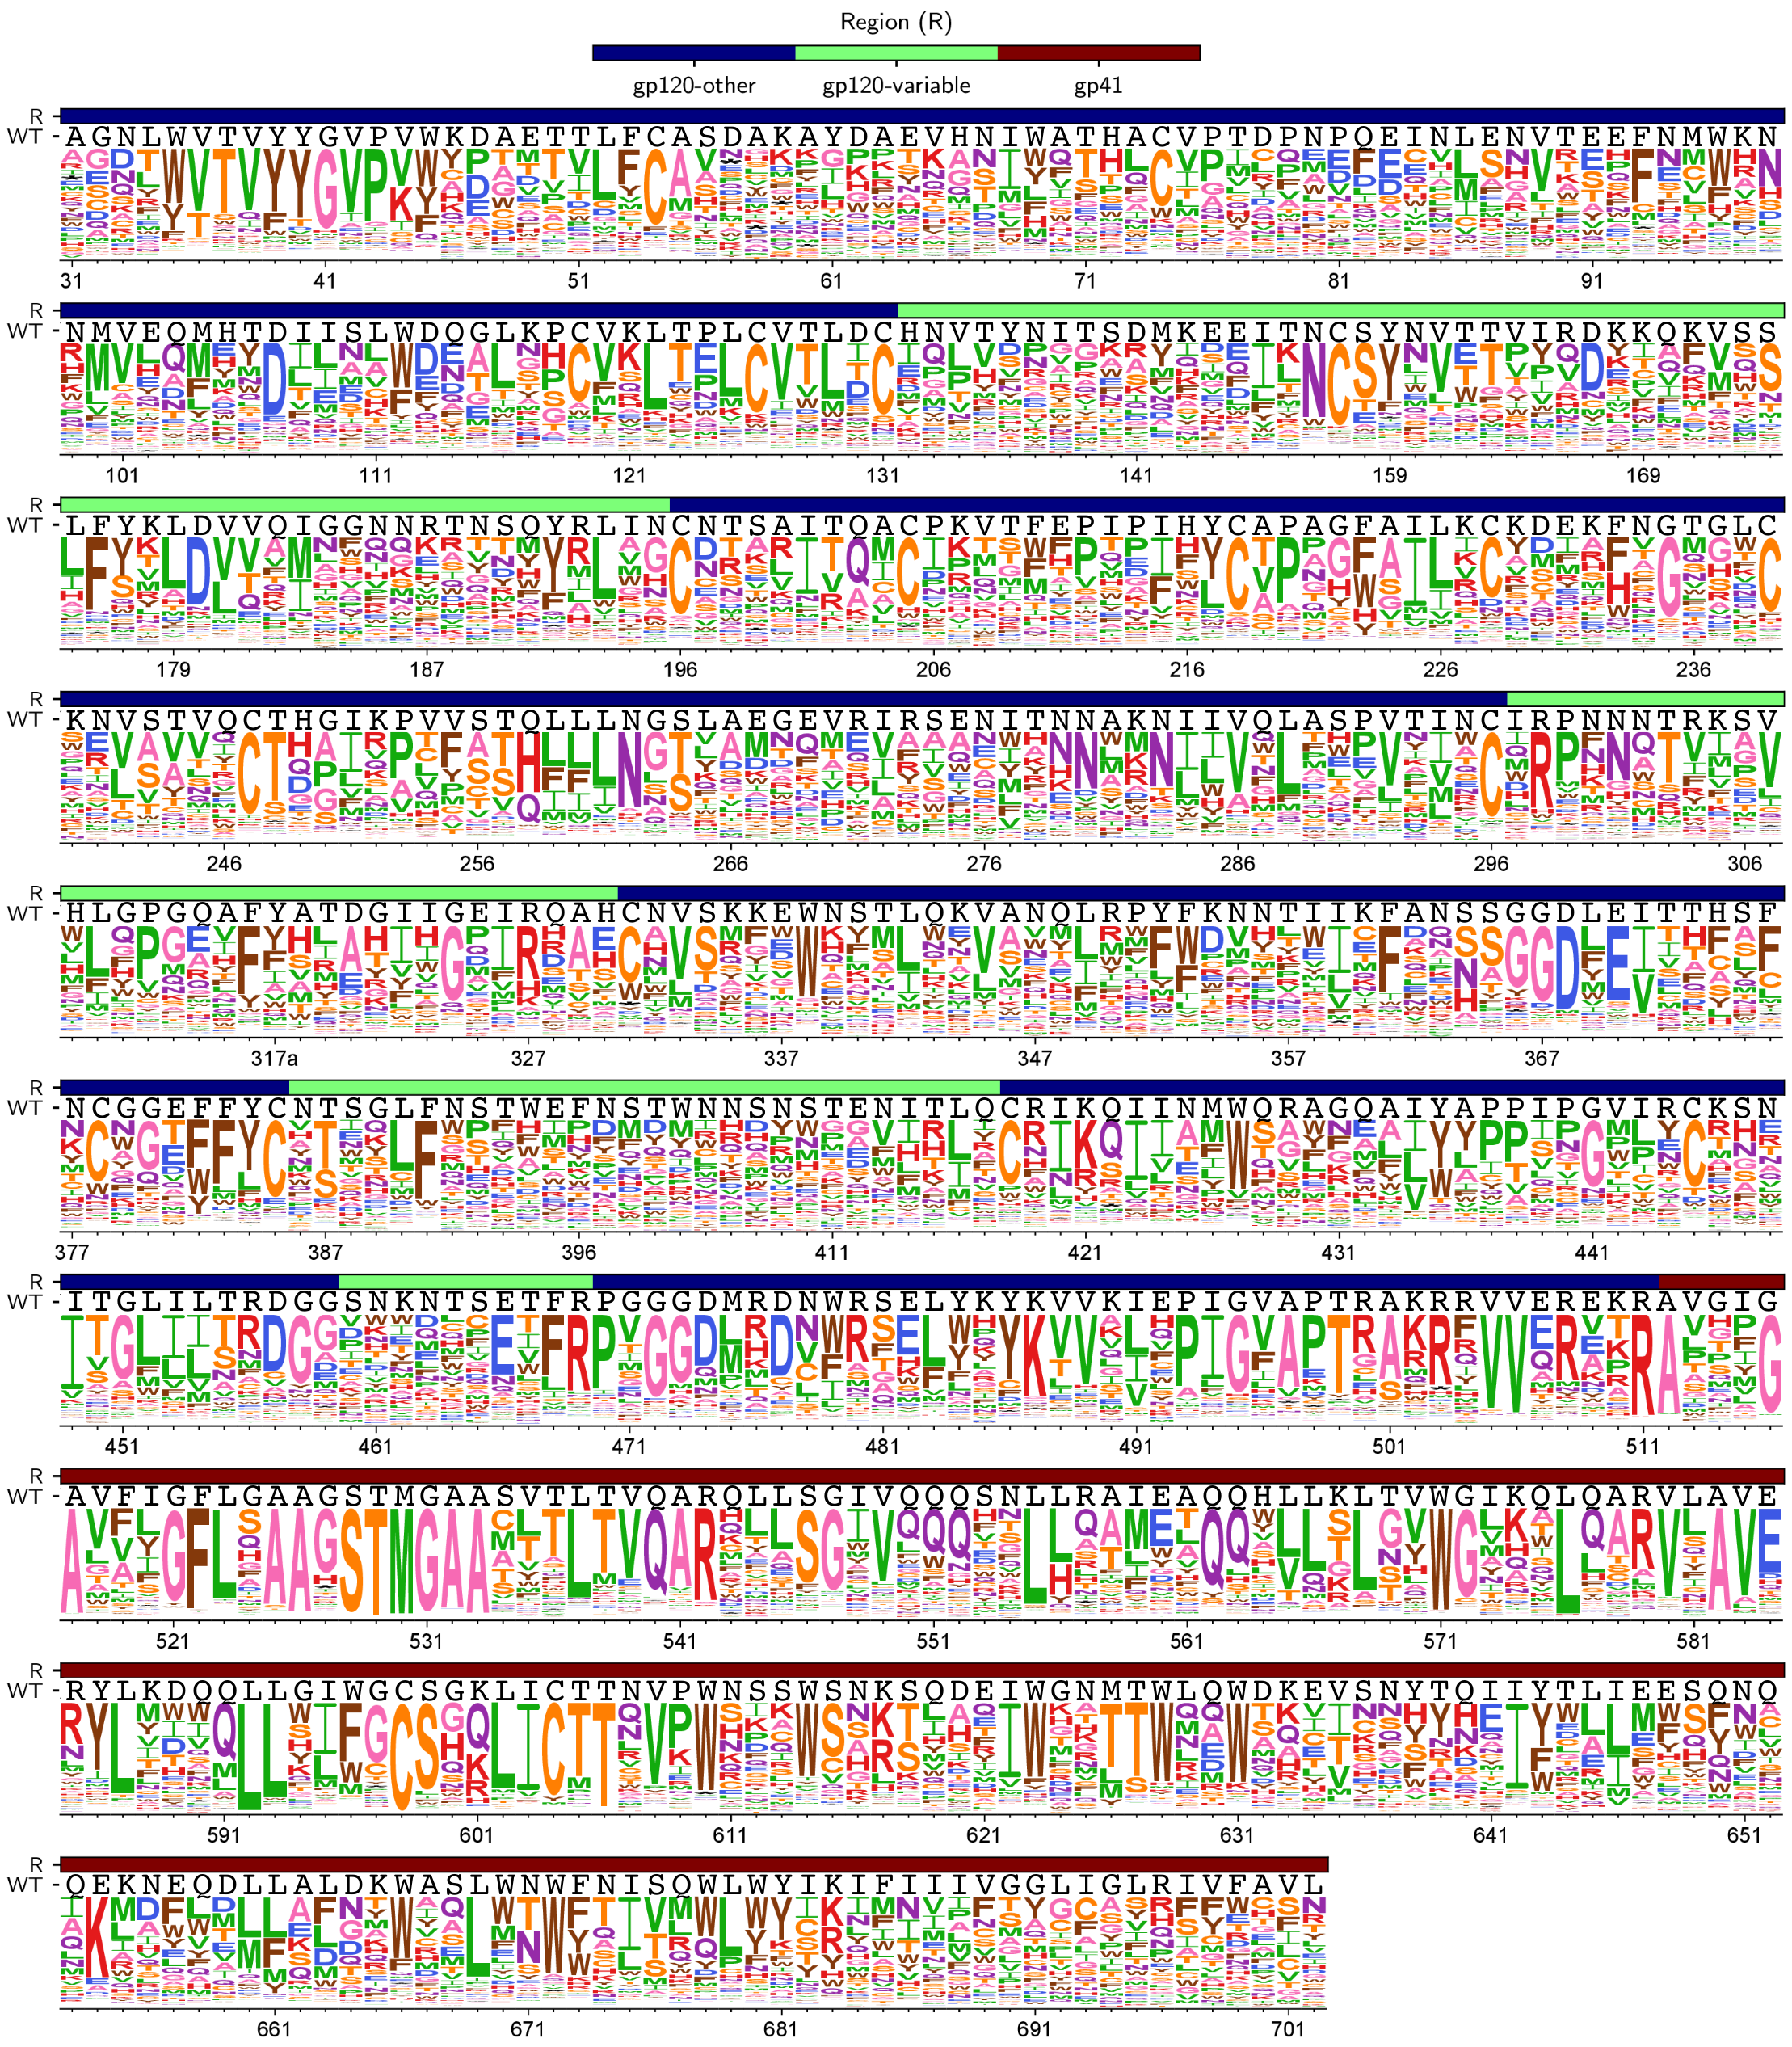
\includegraphics[width=6.5in]{figures/prefs_BF520/prefs_BF520.png}}
\caption{\label{fig:bf520_prefs_logo}
The re-scaled averaged site-specific amino-acid preferences for BF520.
This figure is the same as Fig \ref{fig:bg505_prefs_logo}, but for BF520 instead of BG505.
}
\end{figure}

A supplemental file for each of these and the results for each replicate. This is a lot of files, so you might just make a zip with all eight.

\subsection*{Differences between homologs}

\begin{figure}
\centerline{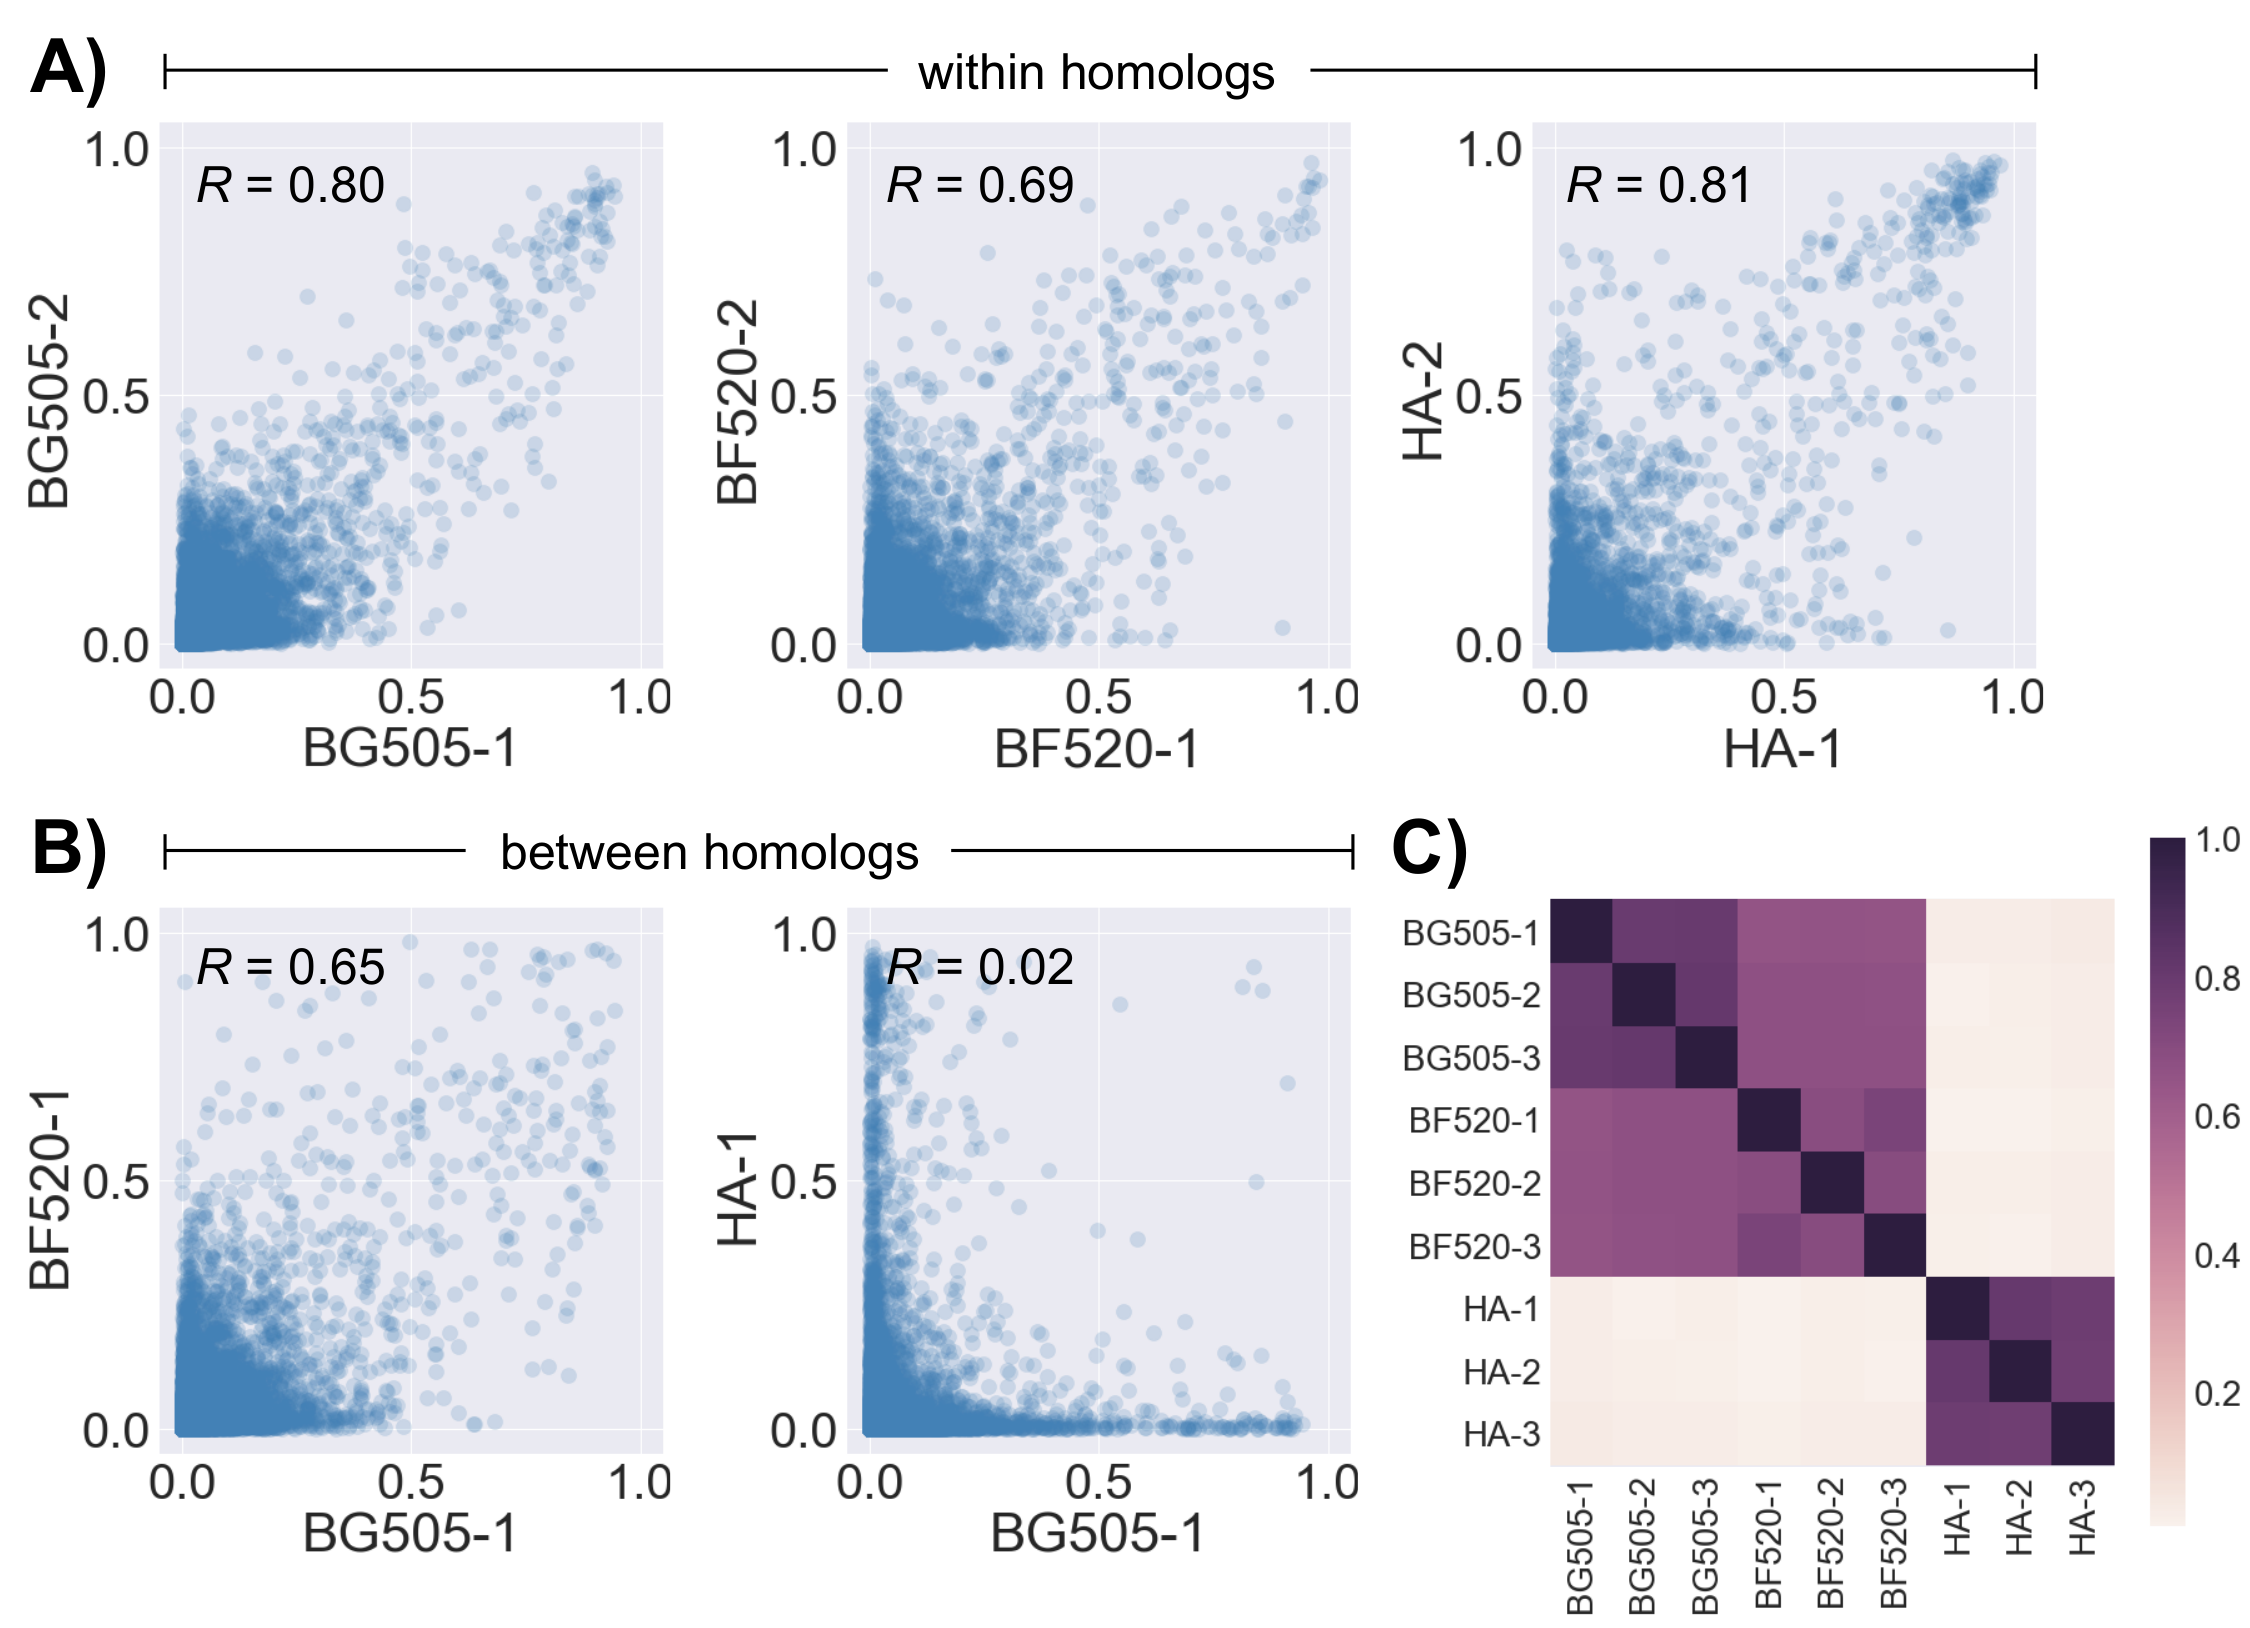
\includegraphics[width=6.5in]{figures/homologs_corr/homologs_corr.png}}
\caption{\label{fig:homologs_corr}
Env's preferences are well correlated between BG505 and BF520.
This figure shows the correlation of the preferences between replicates, both within and between Env homologs.
In this figure, the preferences for each replicate have been rescaled using the stringency parameter for the corresponding homolog from the group-M analysis in Table \ref{tab:phydms}.
We analyzed 616 sites that are shared between homologs and were in readily alignable regions of the group-M multiple-sequence alignment.
As a control, we also compared our estimates of Env's preferences with the preferences of a non-homologous protein -- influenza HA -- across the 480 sites where these proteins overlap in sequential numbering.
{\bf (A)} Plots showing the correlation of preferences between two replicates from the same protein.
Here, differences reflect experimental noise.
{\bf (B)} Plots showing the correlation of preferences between Env homologs, or between BG505 and HA.
Here, differences reflect a combination of experimental noise and biological differences between proteins.
The Env homologs are well correlated, whereas BG505 and HA are not correlated.
{\bf (C)} The heat map shows the Pearson correlation coefficient for all pairwise comparisons of all experimental replicates of each homolog (coefficients are also shown on the correlation plots).
This heat map indicates that the trends in {\bf (A)} and {\bf (B)} hold for all replicates.
}
\end{figure}

\begin{figure}
\centerline{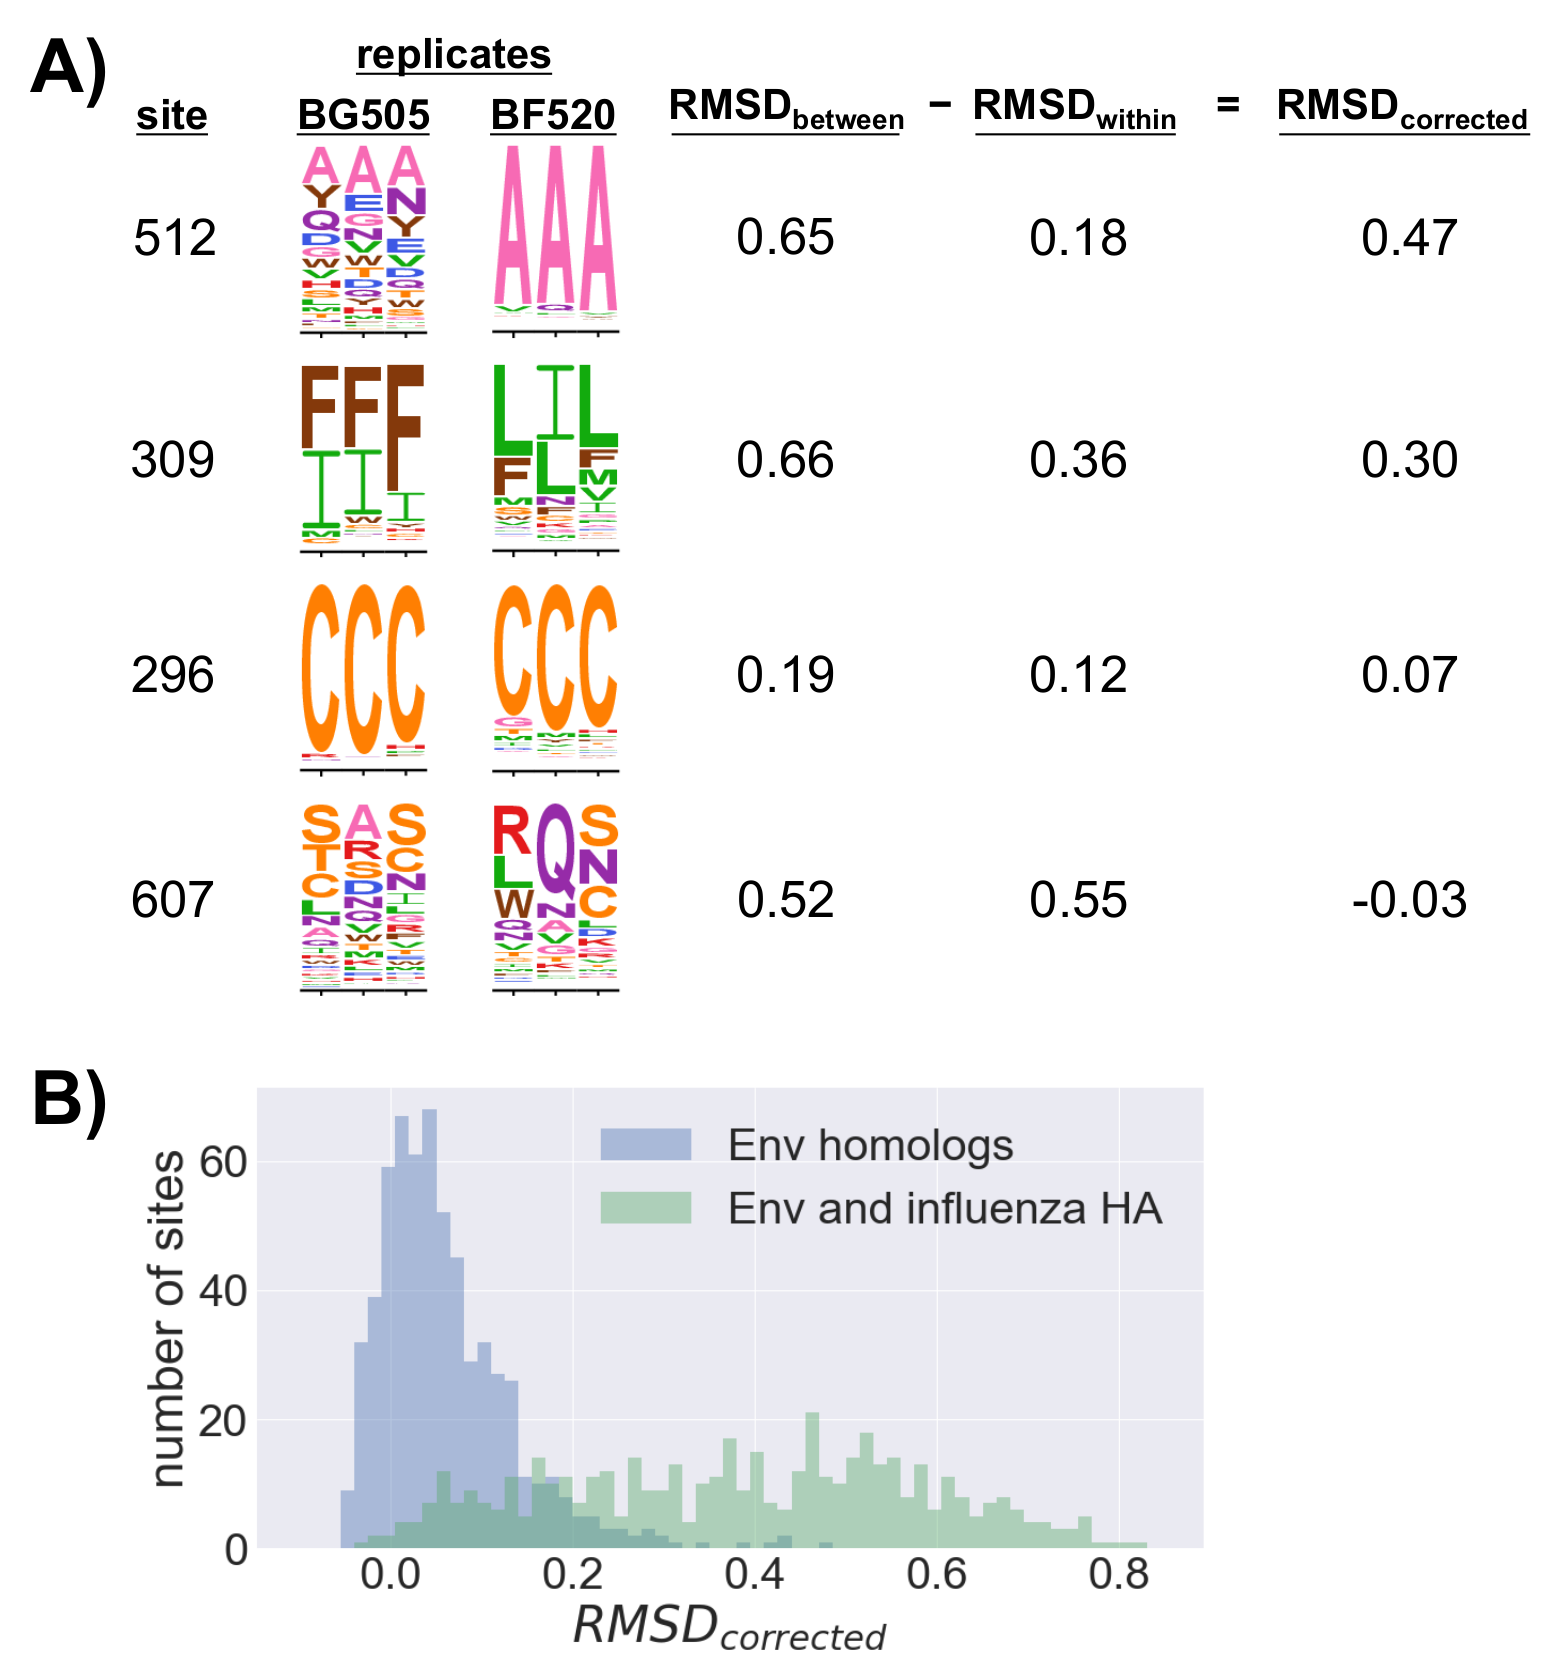
\includegraphics[width=4.5in]{figures/distances/distances.png}}
\caption{\label{fig:distances}
Most shifts in amino-acid preference between Env homologs are small-to-intermediate in effect size after correcting for experimental noise.
We quantified the shift in each site's preferences using a distance metric that corrects for experimental noise, as quantified by experimental replicates.
{\bf (A)} This panel shows how the distance metric is calculated for a subset of sites.
{\bf (B)} The blue histogram shows the distribution of site-specific $RMSD_{corrected}$ values between Env homologs for all 616 sites being compared.
Most sites have a distance greater than zero.
The overlayed green histogram shows the distribution of $RMSD_{corrected}$ values between BG505 Env and influenza HA for all 480 sites that overlap in sequential numbering.
Most site-specific distances in the Env-HA comparison are much larger than the distances in the BG505-BF520 comparison.
}
\end{figure}

Add a supplemental figure showing that the distance metric we use (half sum absolute corrected) is correlated with other distance metrics (e.g., Jensen-Shannon distance).

\begin{figure}
\centerline{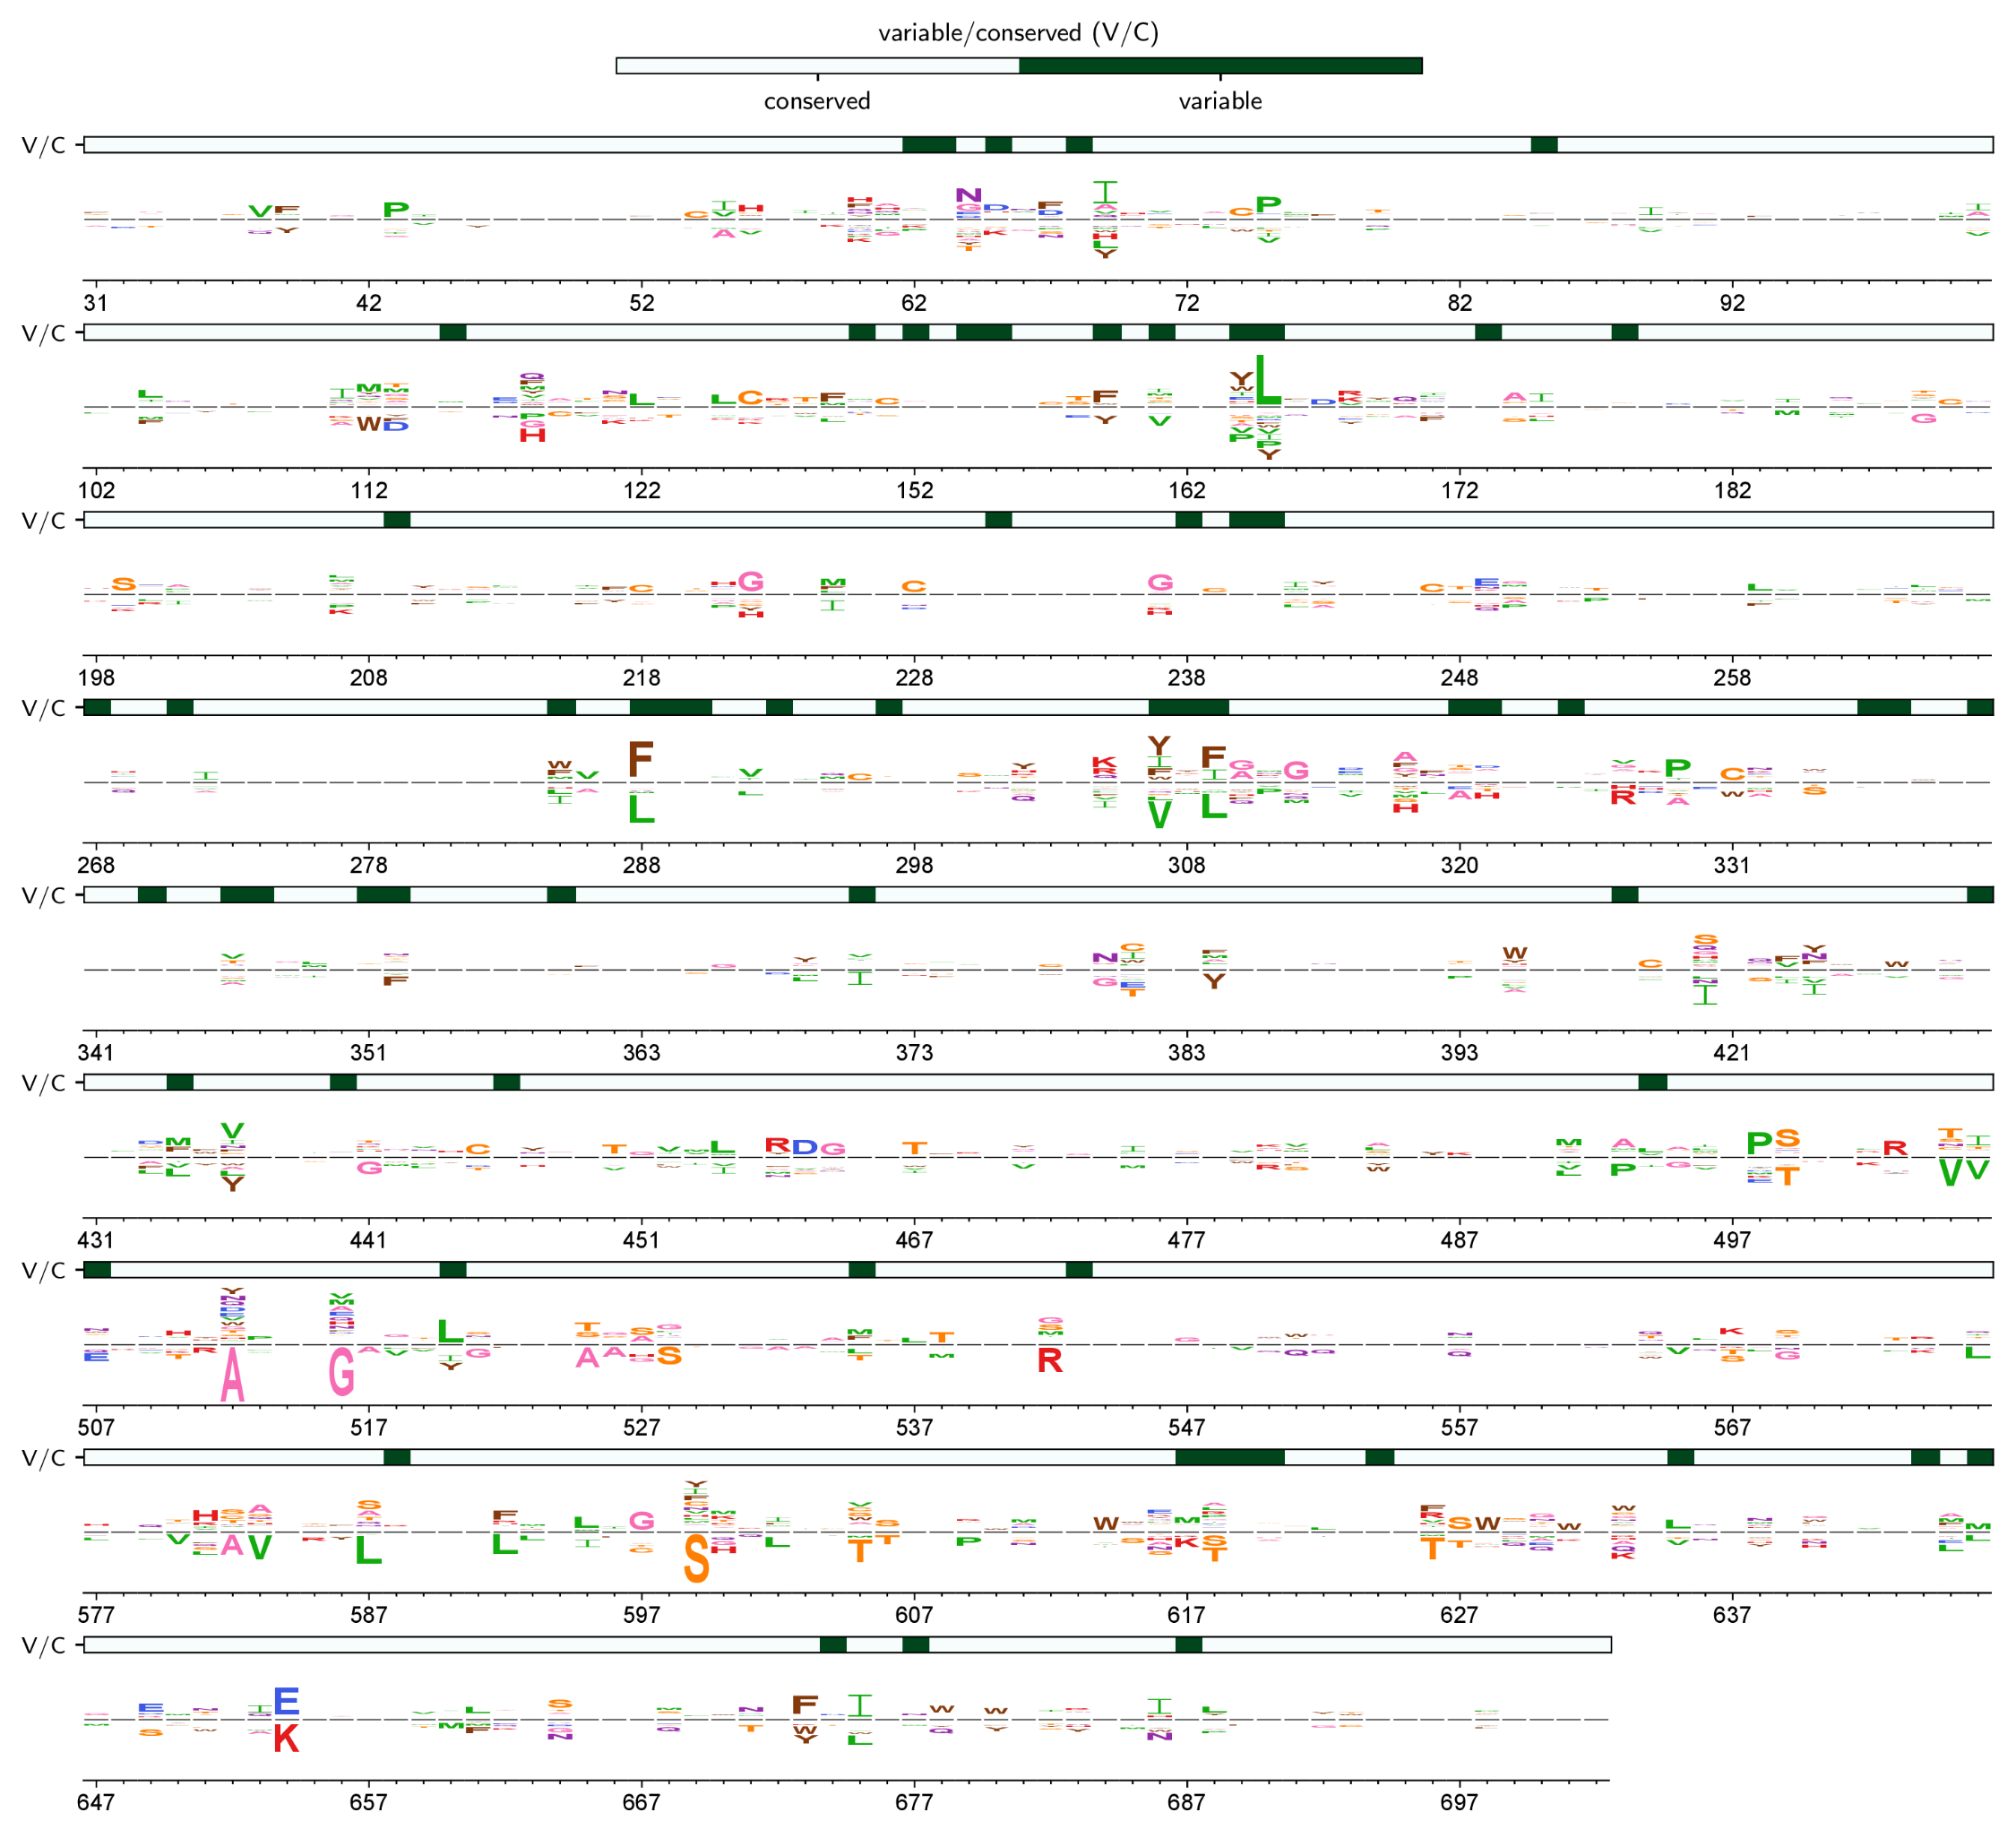
\includegraphics[width=6.5in]{figures/diffs_logo/diffs_logo.png}}
\caption{\label{fig:diffs_logo}
{\bf The difference in Env's site-specific amino-acid preferences between homologs, scaled by site-specific $RMSD_{corrected}$ values.}
This figure shows the estimated preference shift for each amino acid across all 616 sites in Env being compared.
For each site, we plot the difference in the rescaled averaged preferences between homologs ($\Delta\pi_{r,a} = \pi_{r,a}^{BG505} - \pi_{r,a}^{BF520}$), where each site has 20 letters corresponding to the 20 amino acids, and where negative and positive values are shown below and above the central black line, respectively.
Thus, amino acids above the central line are more preferred in BG505, whereas amino acids below the central line are more preferred in BF520.
At each site, we adjusted the total height of the letters in both directions to equal that site's $RMSD_{corrected}$ from Fig \ref{fig:distances}B (i.e., $\sum_{a}| \Delta\pi_{r,a} | = RMSD_{corrected}$).
In effect, the sites with the largest stack heights are the sites where we observe the largest differences, after accounting for noise.
The bar indicates which sites are variable or conserved in amino-acid sequence between homologs.
Note that adjacent sites are not always contiguous in primary sequence, since we masked sites that are either not shared between homologs, or are not readily alignable in the group-M multiple-sequence alignment.
}
\end{figure}

Plot overlays of conserved and variable, and surface versus core?

\subsection*{Validating sites of mutational shifts}
Describe and validate a few of these sites

\subsection*{Looking at how shifts relate to evolution and structure}

\begin{figure}
\centerline{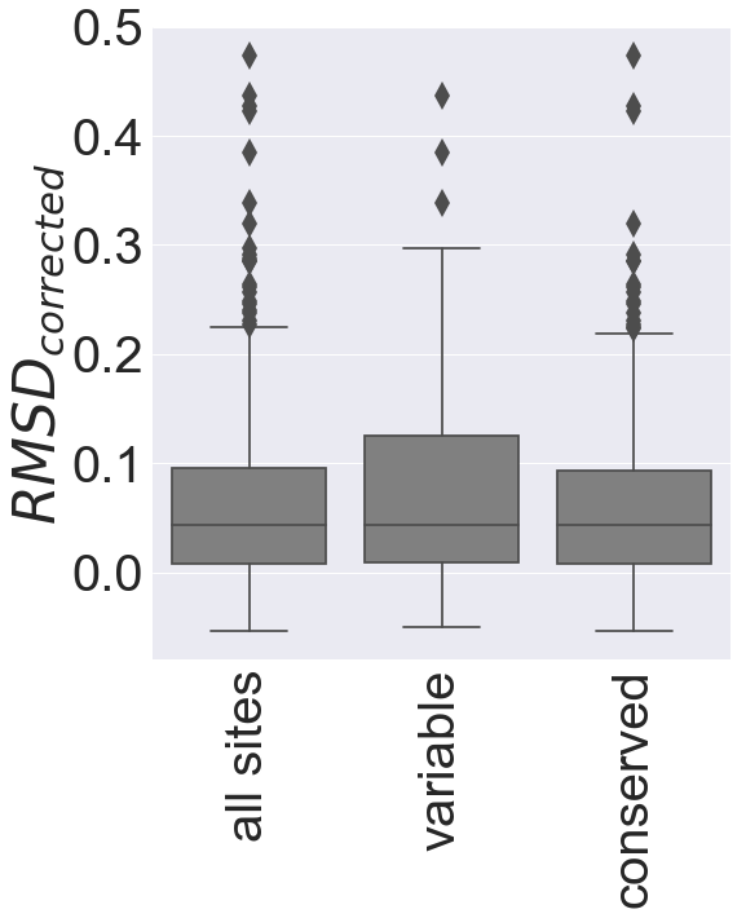
\includegraphics[width=2.5in]{figures/distances_at_subsets_of_sites/distances_at_subsets_of_sites.png}}
\caption{\label{fig:shifts_at_variable_sites}
{\bf The median shift in preferences between Env homologs is similar at variable vs. conserved sites.}
The box plots compare show the shifts at all sites, just sites that differ in wildtype amino acids between BG505 and BF520 (variable), or sites that are conserved between the homologs.
Shifts are quantified by site-specific $RMSD_{corrected}$ values from Fig \ref{fig:ch3_distances}.
The median shift is roughly equivalent for each group of sites.
}
\end{figure}

\section{Discussion}


\section{Methods and Materials}

\subsection*{Sequence alignments}

\section{Acknowledgments}

\nocite{*} % This command displays all refs in the bib file
\bibliography{references.bib}

\section*{Supplementary Material}

\begin{figure}
\centerline{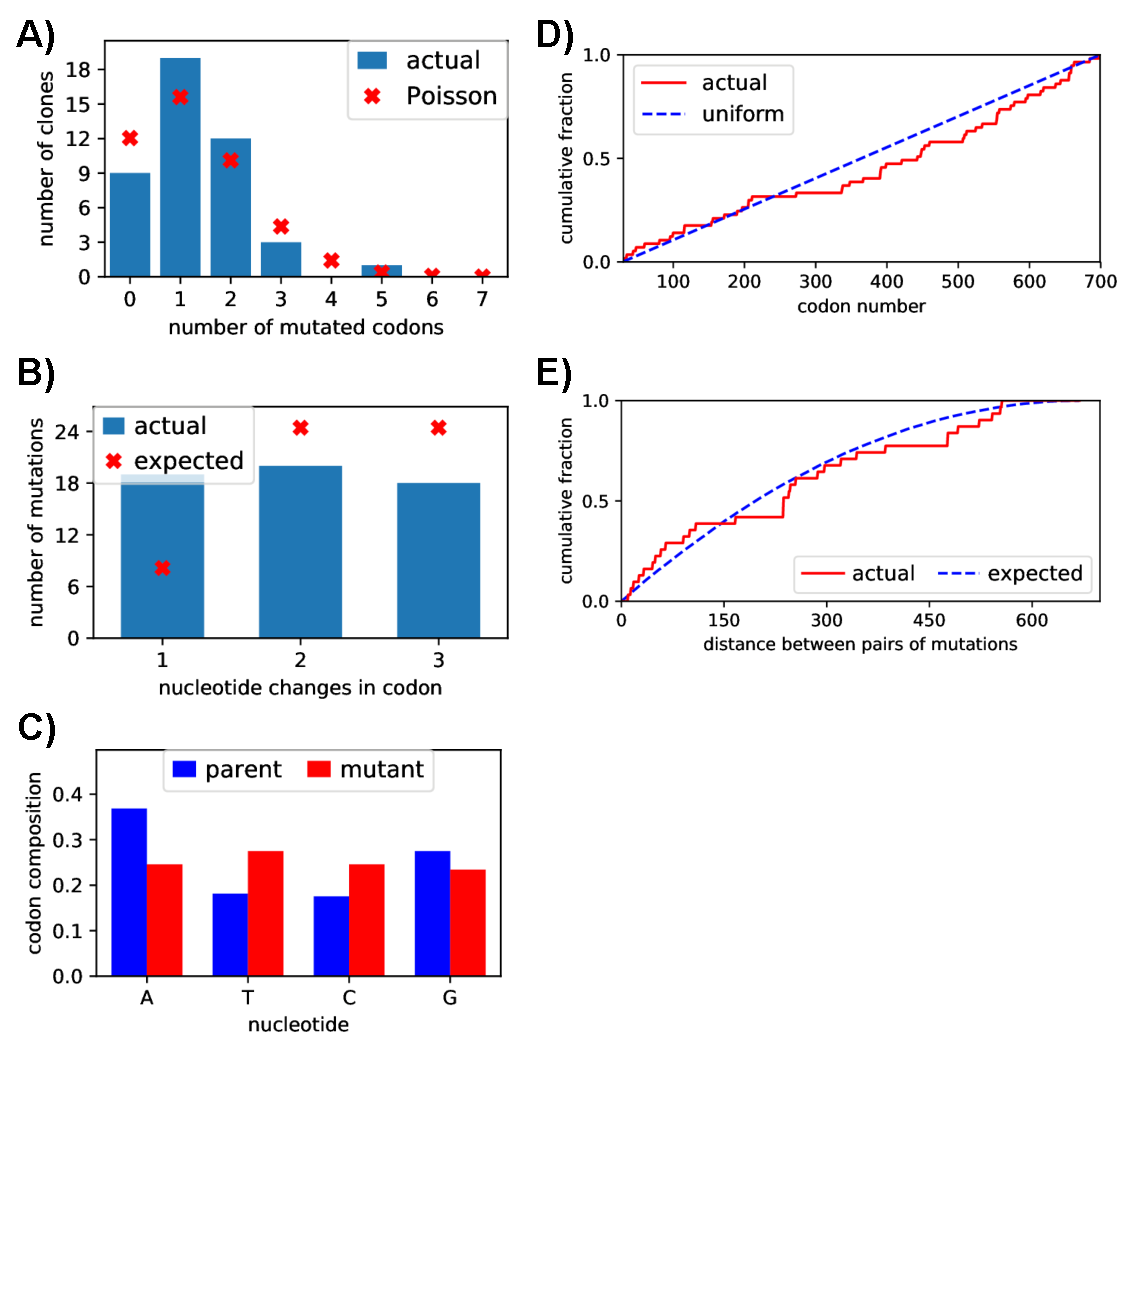
\includegraphics[width=5in]{figures/sanger_sequencing_supp/sanger_sequencing_supp}}
\caption{\label{suppfig:sanger_sequencing_supp}
{\bf Sanger sequencing of the BG505 mutant plasmids revealed that codon mutations were distributed roughly uniformly, with an average of 1.5 mutations per gene.}
We Sanger sequenced 44 clones of BG505 Env.
We sampled these clones roughly evenly from the three replicate mutant plasmid libraries before these libraries had undergone any functional selection. 
{\bf(A)} There was an average of 1.5 mutant codons per clone, with the number of mutations per clone roughly following a Poisson distribution. 
{\bf(B)} The mutant codons had a mix of single-, double-, and triple-nucleotide changes, with an elevated number of single-nucleotide changes than expected.
{\bf(C)} Nucleotide frequencies were fairly uniform in the mutant codons, as expected from random mutagenesis.
{\bf(D)} Mutations were distributed roughly evenly along the mutagenized region of {\it env} (30-699 in BG505 numbering).
{\bf(E)} For clones with multiple mutations, we computed the pairwise distance in primary sequence between each codon mutation and plotted the cumulative distribution of these distances (red line). 
We also simulated the expected distribution of pairwise distances if mutations occurred entirely independently (blue line). 
The observed distribution is close to the expected distribution.
}
\end{figure}

\end{document}
